
\begin{itemize}
    \item Other fields, such as bio-statistics characterize multilevel models not by within- or between-cluster effects, but rather by whether they represent a marginal or conditional-on-the-random-intercept effect. These conceptions are, as almost entirely absent from the psychological literature (e.g., textbooks) on multilevel modeling, indicating the presence of a major divide.
    \item In these fields, it has been long discussed that while fixed slopes in multilevel \textit\textit{linear} models may be interpreted not only as a conditional-on-the-random-intercept effect, but also as a marginal effect. This equivalence is, however, generally not the case for multilevel with non-linear link functions (see shiny app for GLMM with logit link: when the random intercept variance is greater than 0). 
    \item The bio-statistics literature has voiced concerns with the fact that the marginal interpretation cannot be expected to be valid for fixed slopes for non-linear multilevel models. 
    \item As a result, these disciplines tend to favour other methods that can be expected to provide marginal effects, such as Generalized Estimating Equations (GEE), which is a model for clustered-longitudinal data that does not model random effects.
    \item Other disciplines tend
\end{itemize}

% \paragraph{Multilevel Models with binary Predictors and/or Outcomes}

% Across both binary outcomes and predictors, we find that Mundlak's contextual model (L4) and L3 consistently performed best at extraction of the within and contextual effects. The centered predictor only model (L2) performed similarly well for capturing the within effect for continuous outcomes, but did not perform as well for scenarios with binary outcome, in particular for scenarios with continuous predictor (see Figure~\ref{fig:results-within}). Noteworthy, the bias in the within-person effect following from the uncentered predictor only model (L1) when a contextual effect was present, was much greater for the three scenarios other than continuous outcome and predictor (see Figure~\ref{fig:results-within}). This implies that the need for correct specification is all the more important when the predictor or outcome is binary. While L3 and L4 performed best, its performance varied across the four DGMs. For scenarios with binary predictors, estimation of the contextual effect was particularly challenging and further excercerbated by a low number of time points (see Figure~\ref{fig:results-contextual}). For scenarios with binary outcomes, the variability in within and contextual effect estimates is much larger than for continuous outcomes, indicating lower efficiency---that is, precision of an estimator.

% All things considered, L3 and L4 consistently performed the best and the other methods yielded substantially more bias for certain scenarios, implying that standard parametrization methods from the MLM literature generalize well to GLMMs with binary predictors and/or outcomes.

% \paragraph{GEEs and Predictor Parametrization}

% Across all scenarios, we saw great correspondence within each parametrization across the different GEEs working correlation structures, except when the predictor was uncentered (G1). For continuous outcomes, we found that the within and contextual effect estimate in Mundlak's operationalization of GEEs (G4) implementations mirrored that of the GLMM, with neither correlation structure performing clearly superior (see Figure~\ref{fig:results-within}). In addition, for G1 with continuous outcomes, we generally found great resemblance between L1 and the exchangeable structure and systematically different results for the independence structure. For binary outcomes and binary predictor, we find that when there is no unexplained variability in the outcome ($\sigma_u = 0$), the G4 implementations retrieve the two fixed effects just as well as L4 (where the contextual effect was slightly biased), whereas the G2 implementations fail to do so. If this is not the case, the G4 estimates are systematically different from the specified two effects and L4 estimates (see Figure~\ref{fig:results-within} and Figure~\ref{fig:results-contextual}). Similarly, when we have a continuous predictor, the two effects in G4 and G2 are systematically different from the specified effects, L4 estimates and each other (see Figure~\ref{fig:results-within}).

% Thus, out of the GEEs approaches, G4 tended to outperform G1 and G2; and consistently performed very similar to L4 for continuous outcomes, while yielding different estimates for most scenarios with binary outcomes. This suggests that in the scenario with continuous outcomes, GEEs requires explicit separation of effects via predictor parametrization if the within-person effect is the target quantity. When the outcome is binary (i.e. modelled with a logit link), it seems as though altogether different quantities are estimated for the within and contextual effects.

% \paragraph{Summary}

% If the target quantity is the within, between and/or contextual effect and the parametric assumptions are met (as in the current DGMs), the GLMM framework more consistently retrieves these effects. It is important to state that GEEs is not worse, but yields a different estimand in the case of a binary outcome, where the marginal interpretation of the fixed effects no longer holds for the GLMM.

% \newpage
% % \begin{center}
%     \captionof{figure}{Bias in Within-Person Effect for Different Estimation Approaches (with $N = 200, T = 5, \sigma_{X,\text{b}} = 3, \gamma_{01} = 3$)}
%     \begin{subfigure}[b]{\linewidth}
%         \centering
%         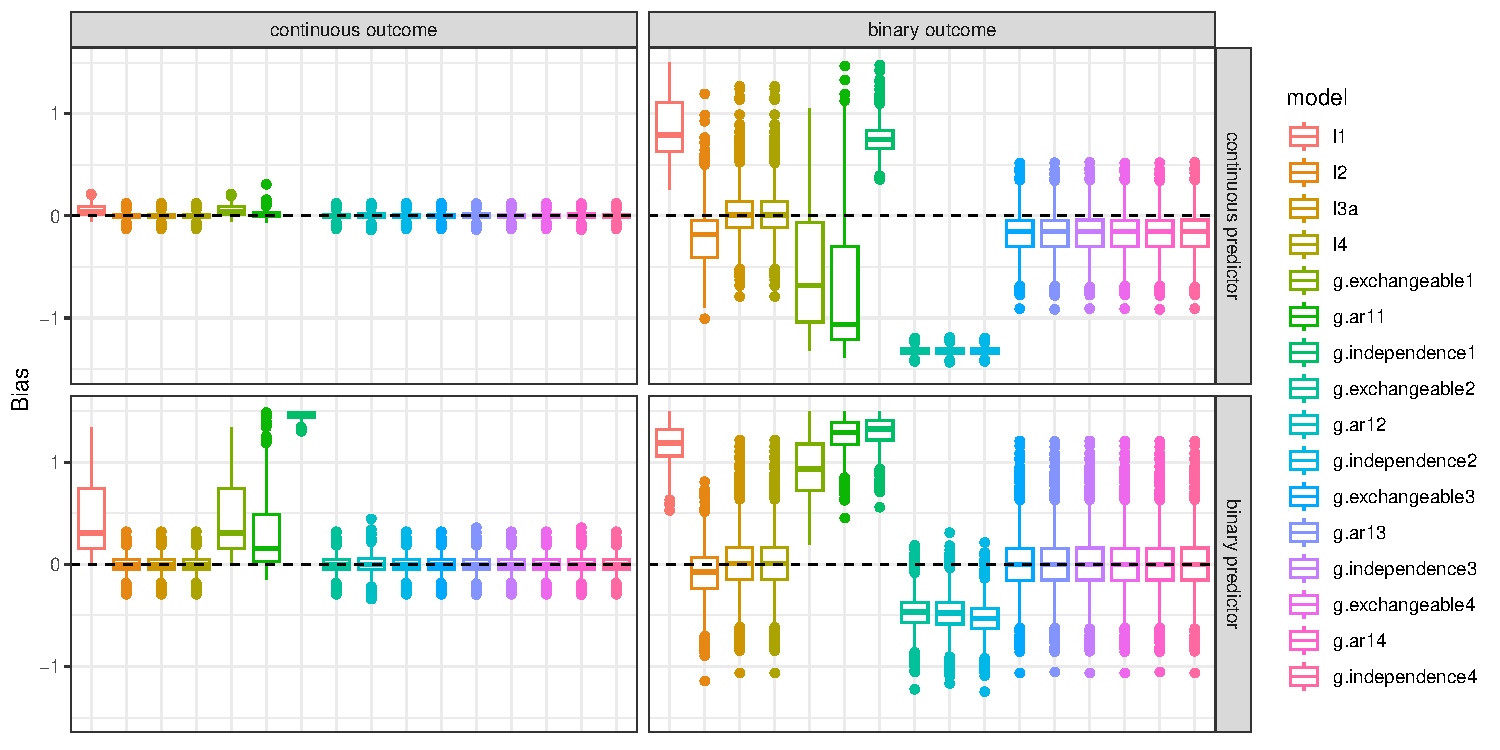
\includegraphics[width=\linewidth, keepaspectratio]{Figures/bias_plot_within_scenario1.pdf}
%         \caption{No Unobserved Heterogeneity ($\sigma_u = 0$)}\label{fig:results-within-scenario1}
%     \end{subfigure}
    
%     \begin{subfigure}[b]{\linewidth}
%         \centering
%         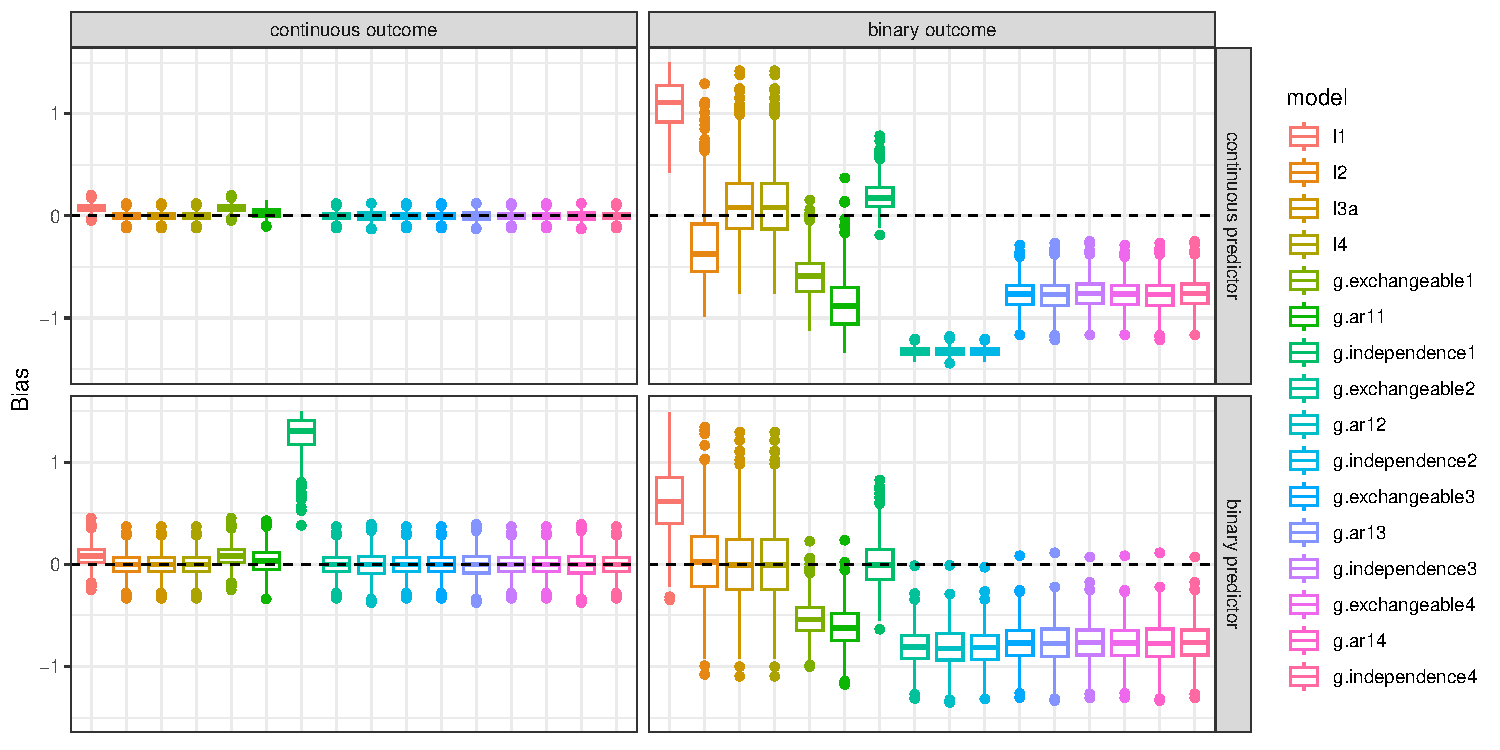
\includegraphics[width=\linewidth, keepaspectratio]{Figures/bias_plot_within_scenario2.pdf}
%         \caption{Large Unobserved Heterogeneity ($\sigma_u = 3$)}\label{fig:results-within-scenario2}
%     \end{subfigure}
%     \label{fig:results-within}
%     % \begin{figurenote}
%     %     \ldots
%     % \end{figurenote}
% \end{center}

% \newpage

\begin{center}
    \captionof{figure}{Bias in Within-Person Effect $\beta_1$ for Different Estimation Approaches for No and Large Unobserved Heterogeneity (with $N = 200, T = 5, \sigma_{X,\text{b}} = 3, \gamma_{01} = 3, \sigma_u = 0, 3$)}
    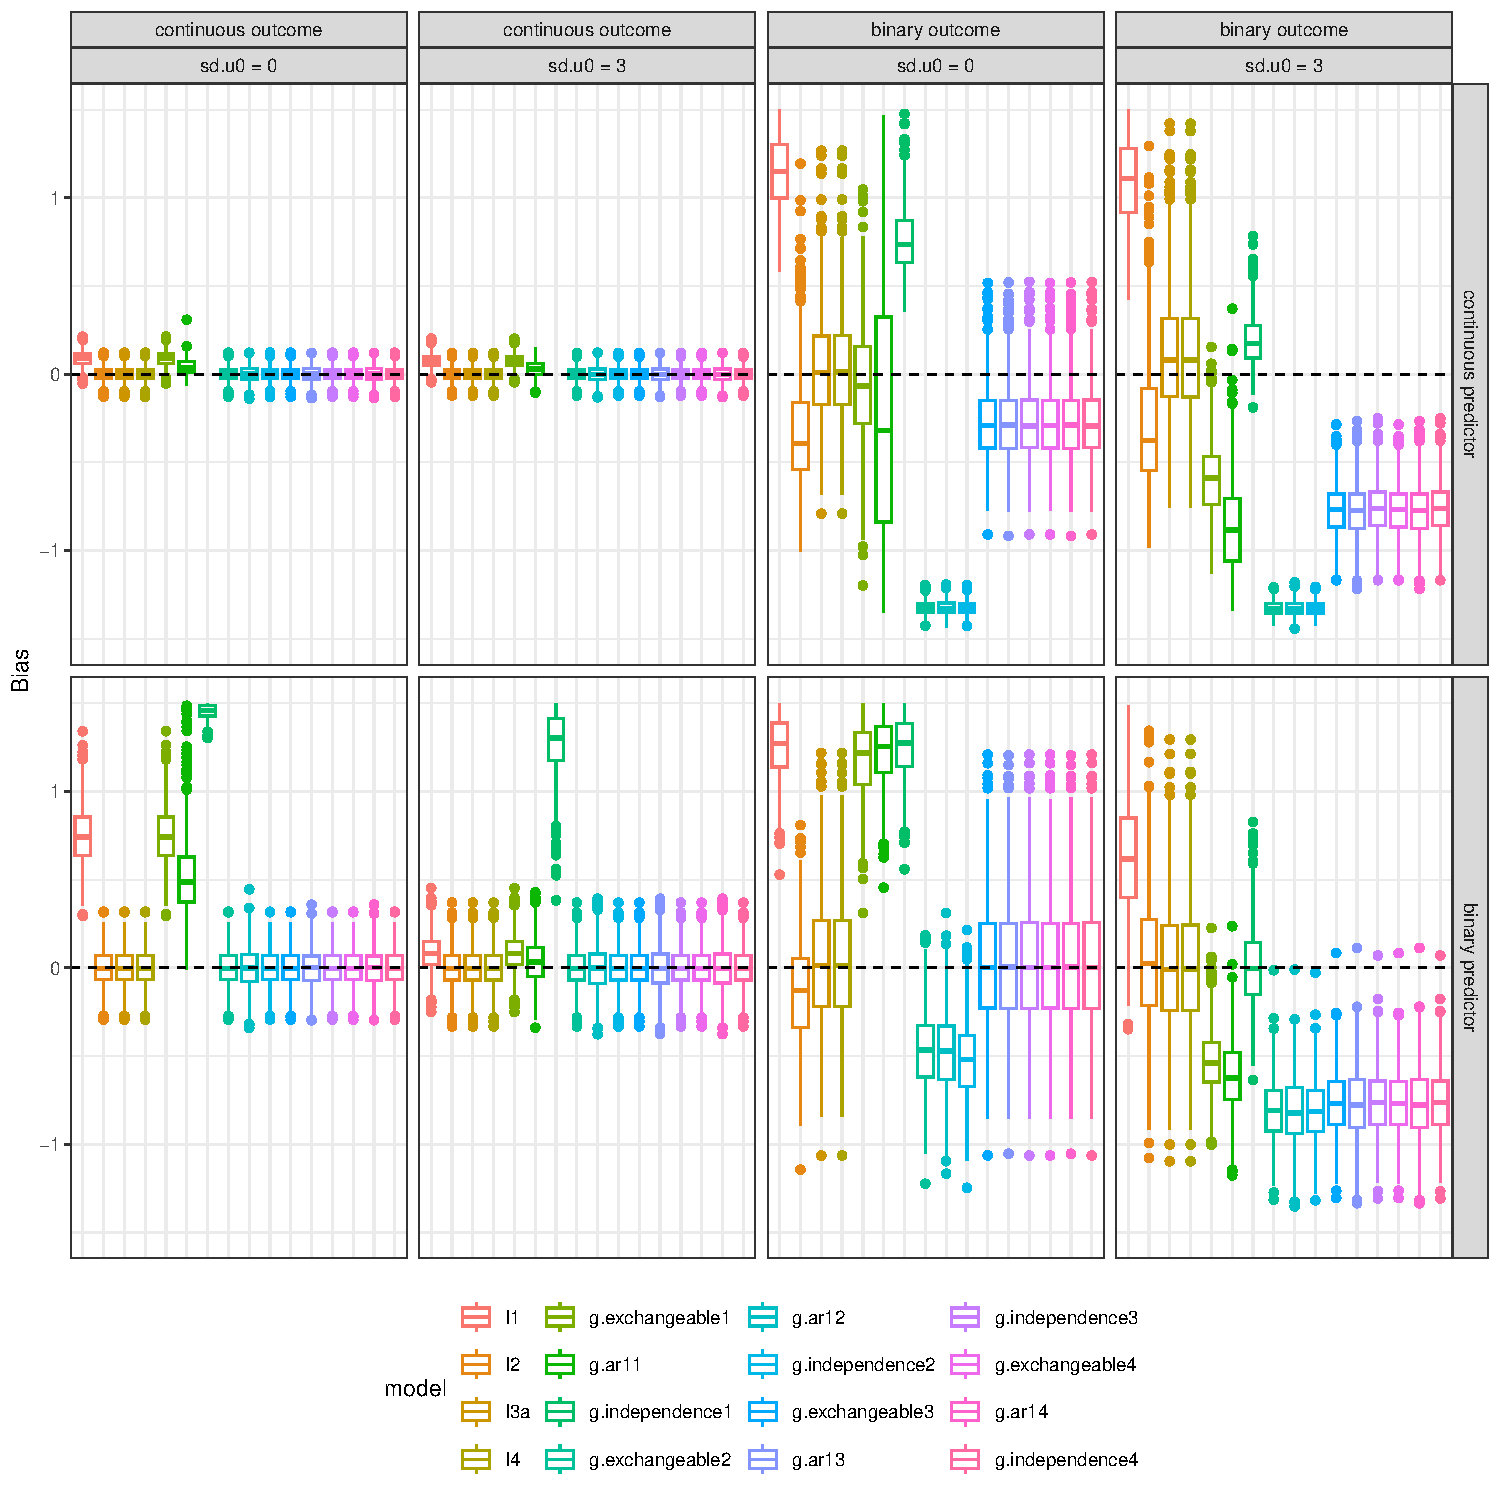
\includegraphics[width=\linewidth, keepaspectratio]{Figures/bias_plot_within_scenario3.pdf}
    \label{fig:results-within}
    % \begin{figurenote}
    %     \ldots
    % \end{figurenote}
\end{center}
% \newpage
% % \begin{center}
%     \captionof{figure}{Bias in Contextual Effect for Different Estimation Approaches (with $N = 200, T = 5, \sigma_{X,\text{b}} = 3, \sigma_u = 0, \gamma_{01} = 3$)}
%     \begin{subfigure}[b]{\linewidth}
%         \centering
%         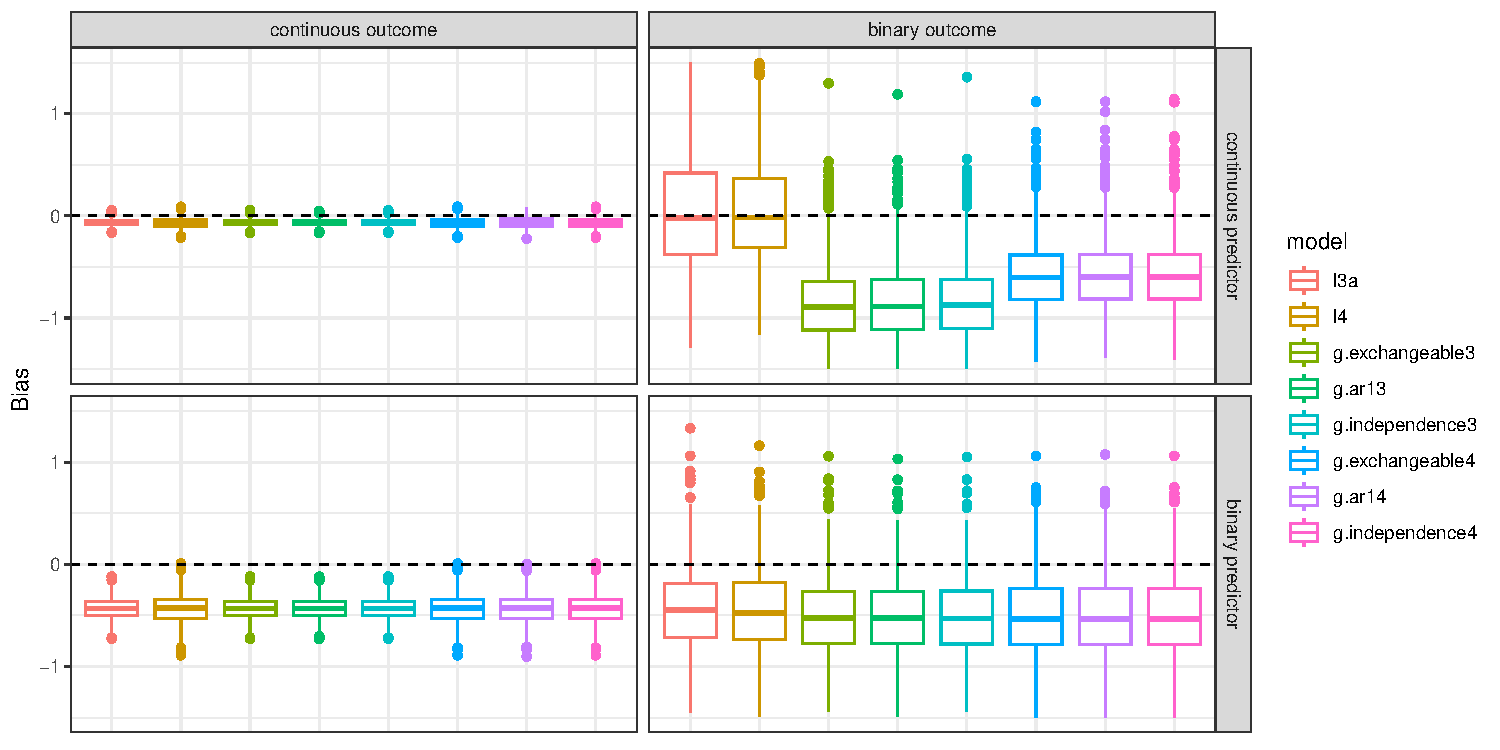
\includegraphics[width=\linewidth, keepaspectratio]{Figures/bias_plot_contextual_scenario1.pdf}
%         \caption{No Unobserved Heterogeneity ($\sigma_u = 0$)}\label{fig:results-contextual-scenario1}
%     \end{subfigure}
    
%     \begin{subfigure}[b]{\linewidth}
%         \centering
%         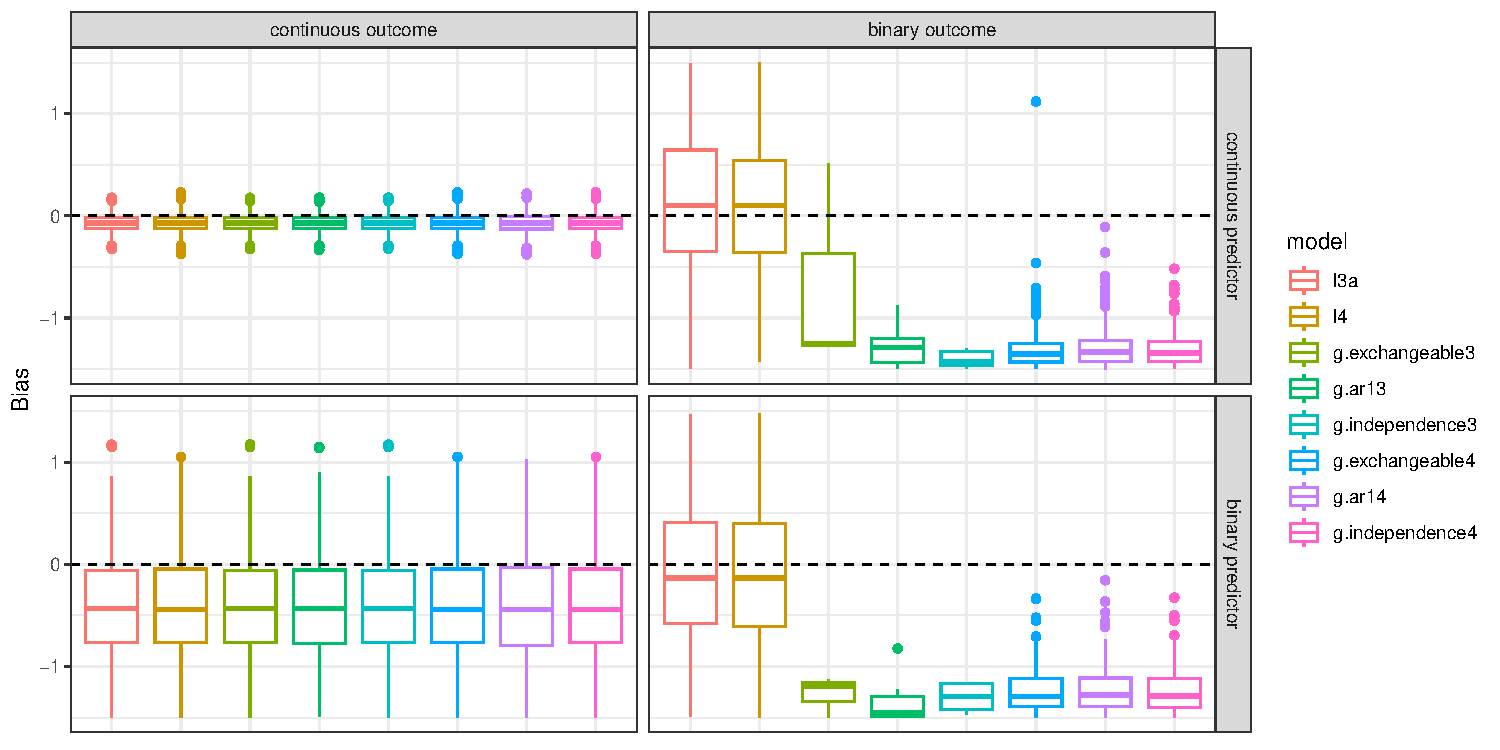
\includegraphics[width=\linewidth, keepaspectratio]{Figures/bias_plot_contextual_scenario2.pdf}
%         \caption{Large Unobserved Heterogeneity ($\sigma_u = 3$)}\label{fig:results-contextual-scenario2}
%     \end{subfigure}
%     \label{fig:results-contextual}
%     % \begin{figurenote}
%     %     \ldots
%     % \end{figurenote}
% \end{center}

% \newpage

\begin{center}
    \captionof{figure}{Bias in Contextual Effect $\gamma_{01}$ for Different Estimation Approaches for No and Large Unobserved Heterogeneity (with $N = 200, T = 5, \sigma_{X,\text{b}} = 3, \gamma_{01} = 3, \sigma_u = 0, 3$)}
    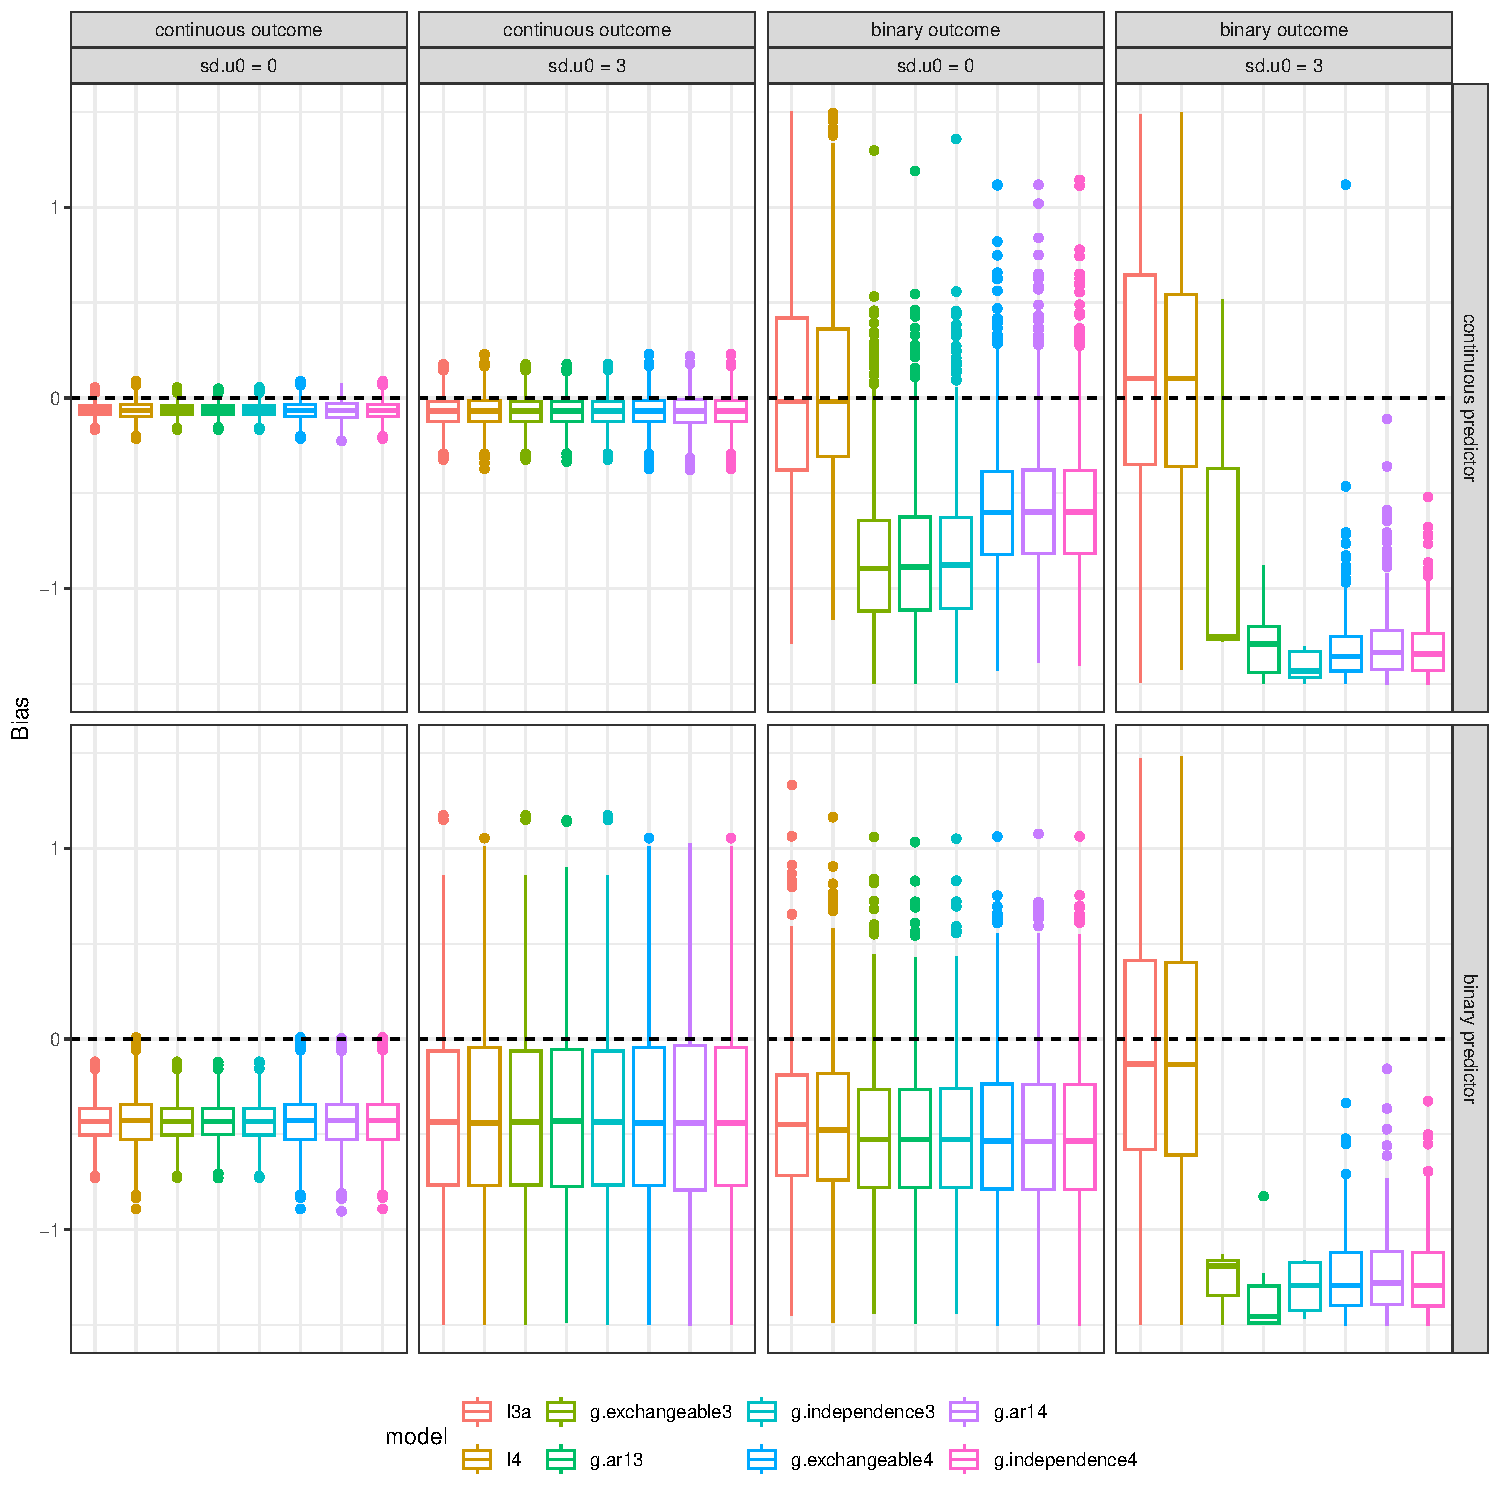
\includegraphics[width=\linewidth, keepaspectratio]{Figures/bias_plot_contextual_scenario3.pdf}
    \label{fig:results-contextual}
    % \begin{figurenote}
    %     \ldots
    % \end{figurenote}
\end{center}